\section{Method 1}

Replace this section with your research methods. The examples below follow
 the text-with-table and four-panel illustration layouts in the official
HKUST(GZ) PhD sample pages~\citep{phd}. All values and curves are synthetic
placeholders, not research findings.

\subsection{A Table in the Text}
Table~\ref{tab:example-results} demonstrates a numbered table with a short
list-of-tables entry, a descriptive caption, and a label placed after the
caption. Define units in the column headings and explain abbreviations in
 the accompanying text.

\begin{table}[htbp]
  \centering
  \caption[Illustrative experimental results]{Illustrative experimental
    results on three synthetic tasks. Scores are percentages; time is in seconds.}
  \label{tab:example-results}
  \begin{tabular}{lrrrr}
    \toprule
    Method & Task A (\%) & Task B (\%) & Task C (\%) & Time (s) \\
    \midrule
    Baseline & 61.2 & 58.4 & 63.7 & 120 \\
    Variant A & 65.8 & 62.1 & 67.3 & 108 \\
    Variant B & 68.5 & 64.9 & 70.1 & 102 \\
    Full method & 72.4 & 69.6 & 74.2 & 95 \\
    \bottomrule
  \end{tabular}
\end{table}

Use \verb|\ref{tab:example-results}| to reference the table rather than
hard-coding its number. This example uses the existing \texttt{booktabs}
package. Its rules and caption placement are illustrative design choices,
not additional university requirements.

\clearpage
\subsection{A Figure with Four Panels}
Figure~\ref{fig:example-panels} follows the official sample's two-by-two
arrangement with panel legends below. The plots are editable vector graphics;
replace each plot with your own PDF or a sufficiently high-resolution image.

\begin{figure}[htbp]
  \centering
  \begingroup
  \pgfplotsset{every axis/.append style={
    width=6.7cm,height=4.8cm,
    tick label style={font=\footnotesize},
    label style={font=\small},
    xlabel={Iteration},ylabel={Score},
    xmin=0,xmax=4,ymin=0,ymax=1,
    xtick={0,2,4},ytick={0,0.5,1},grid=major}}
  \begin{minipage}{0.48\textwidth}\centering
    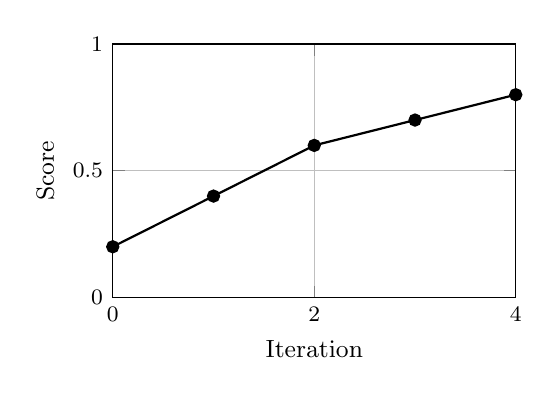
\begin{tikzpicture}\begin{axis}
      \addplot[black,thick,mark=*] coordinates
        {(0,0.2) (1,0.4) (2,0.6) (3,0.7) (4,0.8)};
    \end{axis}\end{tikzpicture}\par (a)
  \end{minipage}\hfill
  \begin{minipage}{0.48\textwidth}\centering
    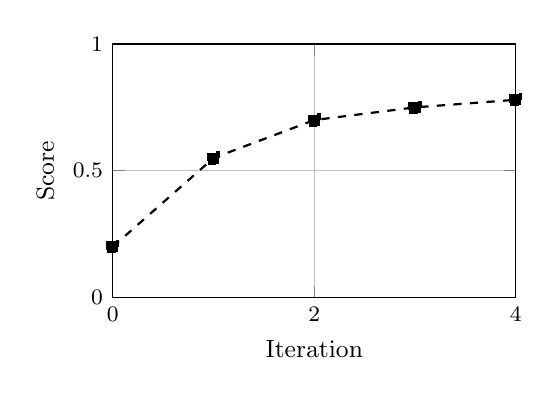
\begin{tikzpicture}\begin{axis}
      \addplot[black,thick,dashed,mark=square*] coordinates
        {(0,0.2) (1,0.55) (2,0.7) (3,0.75) (4,0.78)};
    \end{axis}\end{tikzpicture}\par (b)
  \end{minipage}

  \medskip
  \begin{minipage}{0.48\textwidth}\centering
    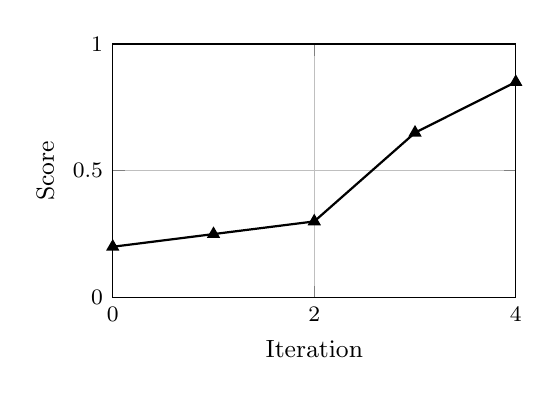
\begin{tikzpicture}\begin{axis}
      \addplot[black,thick,mark=triangle*] coordinates
        {(0,0.2) (1,0.25) (2,0.3) (3,0.65) (4,0.85)};
    \end{axis}\end{tikzpicture}\par (c)
  \end{minipage}\hfill
  \begin{minipage}{0.48\textwidth}\centering
    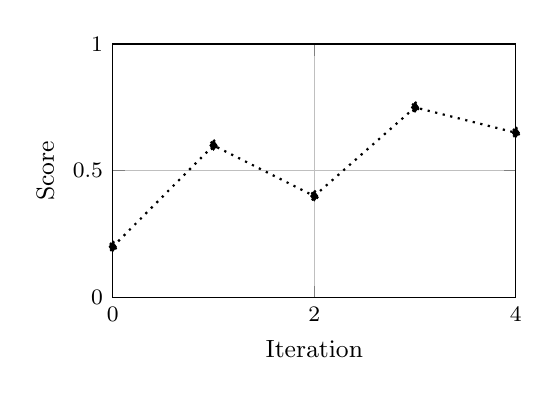
\begin{tikzpicture}\begin{axis}
      \addplot[black,thick,dotted,mark=diamond*] coordinates
        {(0,0.2) (1,0.6) (2,0.4) (3,0.75) (4,0.65)};
    \end{axis}\end{tikzpicture}\par (d)
  \end{minipage}
  \endgroup
  \caption[Illustrative four-panel figure]{Illustrative four-panel figure
    with synthetic trajectories. (a) Steady improvement. (b) Early saturation.
    (c) Delayed improvement. (d) Fluctuating performance.}
  \label{fig:example-panels}
\end{figure}

% For your own image, replace a tikzpicture above with, for example:
% \includegraphics[width=\linewidth]{figures/your-image.pdf}
% Keep \caption before \label so references use the correct figure number.
